\title{Лекции по осям}
\chapter{Лекция 1}
\section{Файловая подсистема Linux}
Файловая подсистема предназначена для обеспечения возможности хранения и доступа к файлам в системе. Это задача которая стоит перед любой файловой системы любой ОС. Unix определил подходы к построению тех или иных модулей системы, к структуризации системы в целом. 

Определение файла из Оксфордского словаря: файл - информация хранимая во вторичной памяти или во вспомог уст с целью ее созранения после заверш отдел задания или преодал огр основного зап устройства (т.н. рабочие файлы). В файле может содержаться любая информация.

Современное определение файла: файл - это любая поименованная совокупность данных, которая хранится во вторичной памяти.*

Определение файловой системы: файловая система - это порядок, определяющий способ организации хранения, именования и доступа к данным на вторичных носителях информации. (Определение состоит из указания задач файловой системы).

Это общие представления о файловой системе.

Рассмотрим обобщенную модель файловой системы. (Из иерархической модели Медника-Донована - на самом высоком уровне файловая система). Аналогично любая файловая система имеет иерархическую структуру. Это связано с разными уровнями этой файловой системы так как различные задачи, которые решает файловая система, выполняются на разных уровнях операционной системы.

Именование файлов (символьный уровень) - это самый высокий уровень файловой системы. Он позволяет пользователю в удобной форме задавать имена файлов и искать их в каталогах. Но файл хранится на физическом уровне (является внешним), значит на нижнем уровне доступ к нему осуществляется с подсистемой ввода-вывода, так как, чтобы считать файл необходимо обратиться к внешнему устройству.

\begin{figure}[H]
	\center{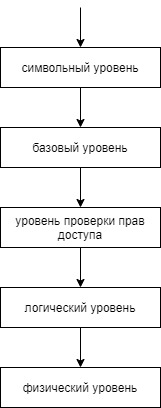
\includegraphics[scale=0.6]{-1}}
\end{figure}

В системе у файла существует полное имя и короткое имя. Система всегда оперирует полным именем. В различных системах имеются отличия в представлении этого имени (в Windows оно начинается с имени логического диска, в Linux - с корневого каталога).

В Unix имя файла не является его идентификатором. В системе файл идентифицируется номером inode'а. Inode - (фактически) дескриптор файла. Первые два уровня определяют именование файла в системе (см рис 1).

Затем модуль проверки прав доступа. (Важнейшая задача ос - контроль прав доступа read/write/execute).

Логический уровень. В данном случае файл похож на программу. Любая программа считает, что она начинается с нулевого адреса. В программе находится смещение. Логическая организация файла начинается с нуля.

Физический уровень. Файл хранится на внешнем устройстве - это уже подсистема ввода-вывода - это уже прерывания. На этом уровне осуществляется учет особенностей организации внешнего устройства.

Дисковые устройства на сегодняшний день являются единственными блочными устройствами (и флэш-память). Все остальные устройства - символьные.

Это самое общее представление уровней файловой системы.

В UNIX Linux имеется существ отличия в системе для работы с файлами.

В UNIX для работы с файлами организовано через интерфейс, который называется VFS/vnode (Virtual file system/virtual node).

В Linux VFS не определена структура vnode. Это сделано для того, чтобы обеспечить широкую поддержку различных файловых систем без перекомпиляции ядра.

\begin{figure}[H]
	\center{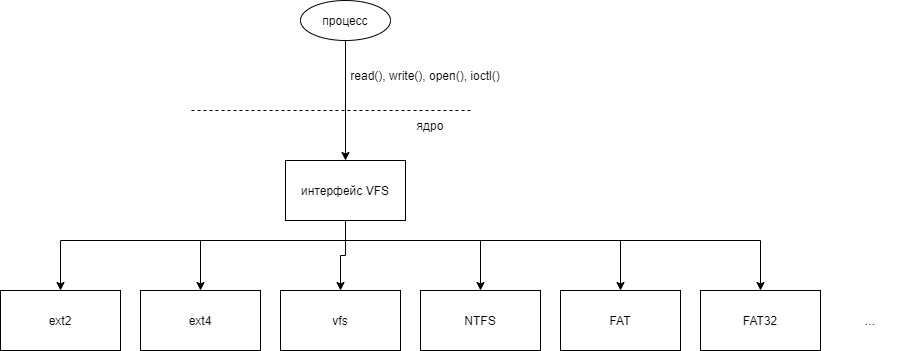
\includegraphics[scale=0.6]{-2}}
\end{figure}


\begin{figure}[H]
	\center{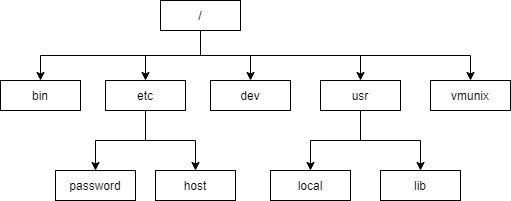
\includegraphics[scale=0.6]{-3}}
\end{figure}

Характерное для UNIX/Linux дерево каталогов.


\begin{figure}[H]
	\center{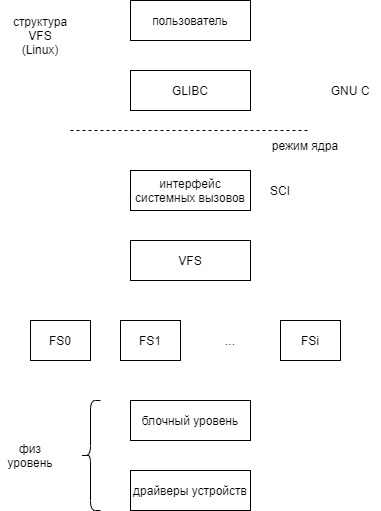
\includegraphics[scale=0.6]{-4}}
\end{figure}

Для Linux важными являются аббревиатуры GNU C и SCI (System call interface / Standard system call interface).


\begin{figure}[H]
	\center{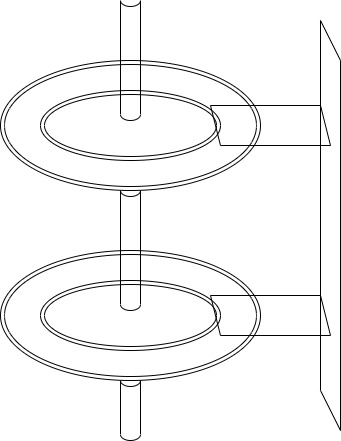
\includegraphics[scale=0.6]{-5}}
\end{figure}

Магнитные диски.

Современные файловыми системами поддерживаются так называемые очень большие файлы. Проводя аналогию с управлением памятью (таблицами страниц), обеспечивается хранение файлов в разброс, они не занимают непрерывные адреса в памяти. Обеспечивается возможность хранения информации из одного и того же файла и это обеспечивается хранением соответствующей информации, а именно адресов блоков.

Такая возможность в ОС юникс линукс реализуется за счет того, что в состав системы входит "слой абстракции" над собственным низкоуровневым интерфейсом файловой системы. Для этого VFS предоставляет общую файловую модель, которая способна отображать общие возможности и "поведение" любой возможной файловой системы. Такой уровень абстракции работает на основе базовых концептуальных интерфейсов и структур данных, которые поддерживаются конкретными файловыми системами. Фактический код любой файловой системы скрывает детали реализации непосредственной работы с данными, организованными в файлы. А именно, предоставл в распоряж польз как правило набор API, таких как открыть файл, прочитать файл, записать в файл, удалить файл, переименовать файл и т.д. Любая файловая система поддерживает такие понятия как файл, каталог и опять же, действия опред над файлами (уже перечисленные). Это можно представить себе следующей абстракцией.


\begin{figure}[H]
	\center{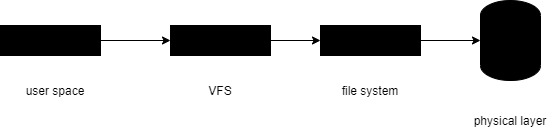
\includegraphics[scale=0.7]{-6}}
\end{figure}

VFS предоставляет общую файловую модель, которую наследуют низлежащие файловые системы, реализуя действия для различных Posix API.

Системный вызов write() сначала обрабатывается общим системным вызовом sys\_write(), который определяет фактический способ записи, характерный той фс, на которой находится файл. Затем общий системный вызов sys\_write() вызывает метод конкретной фс для того, чтобы выполнить запись данных на физический носитель. То есть, VFS (как любая фс) скрывает особенности работы с конкретным физическим устройством.

\section{Организация VFS в Linux}
Внутренняя организация VFS построена на 4-х структурах:

1. Суперблок (superblock)\\
2. Индексный узел (inode)\\
3. Запись каталога (dentry)\\
4. Файл (file)\\

Есть диаграмма связи этих структур.


\begin{figure}[H]
	\center{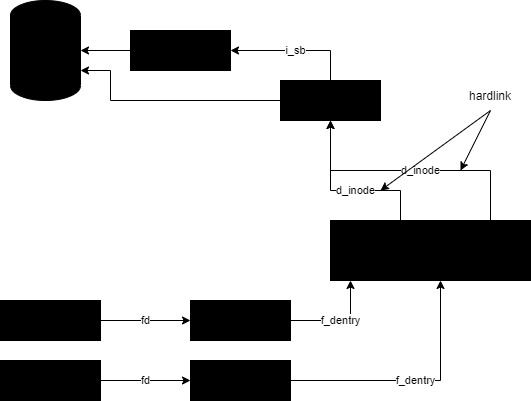
\includegraphics[scale=0.6]{-7}}
\end{figure}

Система различает файл находящийся на диске (его описывает inode) и открытый файл (его описывает struct file) это и показано на рисунке. Показана связь всех 4 структур.

Показано, что 2 процесса открыли файл (один и тот же с разными именами). У него (файла) 1 inode. Очевидно, чтобы обесп доступ к этому файлу в системе имеется struct dentry (сокращение от directory entry) -- обеспечивает работу с каталогами.

Структура superblock в VFS описывает конкретную подмонтированную файловую систему. Т.е. файловую систему, которая находится во внешней памяти, которая располагается на внешнем носителе (подмонтированная).

f\_dentry, dinode, i\_sb - это не идентификаторы, это имена полей соответствующих структур. В struct file есть поле dentry, которая ссылается на структуру, описывающую соответствующий каталог и т.д.

Любой файл хранится в (=принадлежит) конкретной (рабочей, т.е. определенной на диске) файловой системе.

\section{Суперблок}
Суперблок - это контейнер для высокоуровневых метаданных о файловой системе.

Суперблок - структура, которая должна находится на диске, тк эта стр опис фс. Для надежности он хранится в нескольких местах диска. В этой структуре хранятся управляющ параметры фс, такие как суммарное число блоков, свободное число блоков, корневой inode и т.д.

В системе сущ суперблок на диске и суперблок в оперативной памяти. Суперблок на диске хранит информацию необходимую системе для доступа к физическому файлу, т.е. хранит информацию о структуре файловой системе. Суперблок в памяти предоставляет информацию, необходимую для управления смонтированной файловой системой. При этом в системе имеется связный список - struct list\_head superblocks (хранит информацию обо всех подмонтированных файловых системах). Эта структура определена в <linux/fs.h>.

\section{Монтирование}
В дерево файлов и катагов входят отдельн ветви, которые формируются разными фс. Для Юних определено подключение различных файловых систем в дерево каталогов и это действие получило название монтирование.

Монтирование - система действий, в результате которых файловая система устройства становится доступной т.е. можно получить доступ к информации, которая хранится на устройстве.

Базовая форма команды mount принимает на вход 2 параметра: имя устройства (или какого-то другого ресурса, которая содержит монтируемую фс) и точку монтирования. Могут присутствовать ключи - тип файловой системы, опции файловой системы.

mount ключи -t тип\_фс -o опции\_фс устройство каталог(=точка\_монтирования)

\chapter{Лекция 2}
\section{Монтирование и файловые системы}
Путь файла начинается с корневого каталога, который обозначается /. Монтирование - система действий, в результате которой файловая система становится доступной. Для монтирования требуются права и привелегии пользователя. Для монтирования используется команда mount, имеющая следующий синтаксис:\\\
mount ключи -t тип\_файловой\_системы -о опции\_файловой\_системы устройство каталог\_назначениея.\\

Для размонтирования приеняется команда unmount:\\
unmount ключи -t тип\_файловой\_системы -о опции\_файловой\_системы\\

Кроме основной команды существуют дополнительные команды, в которых например может указываться имя файловой системы, например mount\_nfs (Network File System). Если подмонтирована файловая система windows, то mount\_ntfs.

Наиболее часто в команде mount используется два параметра - имя устройства, или другого ресурса, который содержит монтируемую файловую систем и точку монтирования. 

Точка монтирования - каталог к которому подмонтируется файловая система. Точка монтирования должна существовать, иначе возникнет ошибка. 

Когда файловая система смонтирована в существующую директорию, все файлы и поддиректории этой смонтированной файловой системы становятся файлами и поддерживают точку монтирования. 

Если директория точки монтирования содержала в себе какие-либо файлы и поддиректории, то они не теряются, а становятся невидимыми. 

Иногда может оказаться нужным явно указывать при монтировании тип файловой системе. Для этого в команде mount используется опция -t. Это нужно для того, чтобы отследить попытку монтирования файловой системы, использующую новый тип. Unix/Linux могут поддерживать большое количество файловых систем. Существует структура, описывающая тип файловой системы. 

Рассмотрим пример:\\
\# mount /dev/sda1 /mnt - опции -t -o отсутствуют, данная команда пробует монтировать раздел sda1 с файловой системой ext3 в каталог /mnt в режиме только чтения. Если в системе нет библиотек для работы с той или иной файловой системой, или система в указанном разделе не является ext3, будет выдано сообщение о невозможности монтирования. 

Если требуется включить режим записи, то необходимо добавить \# mount -o rw /dev/sda1 /mnt.

\begin{figure}[H]
	\center{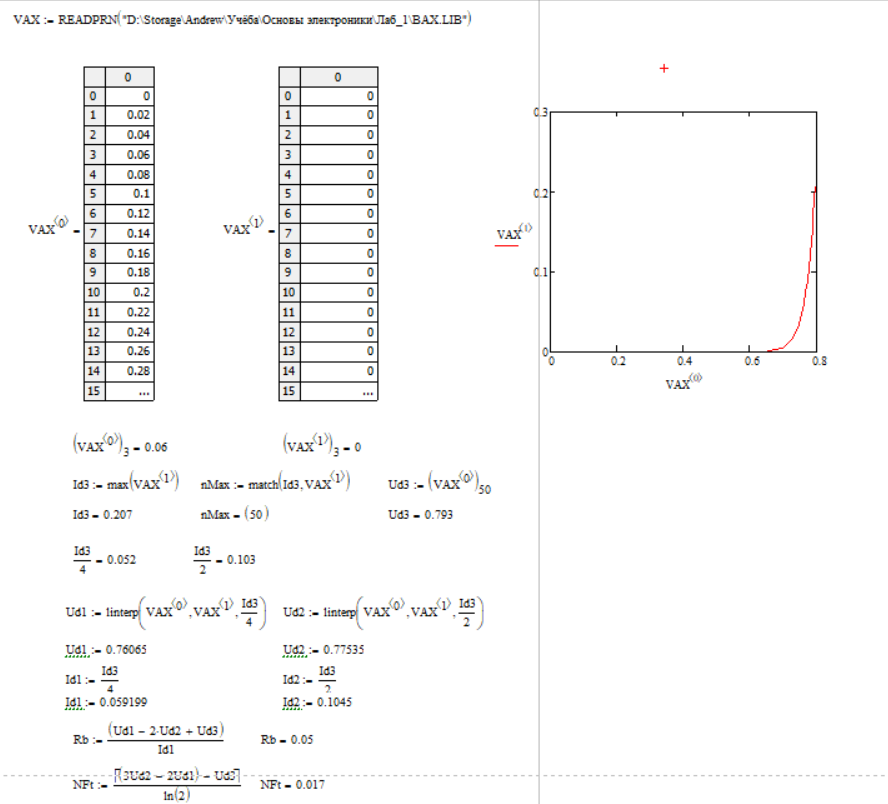
\includegraphics[scale=0.4]{0}}
	\caption{Схема работы файловой системы}
\end{figure}

Структура superblock предназначается для подмонтированных файловых систем. Данная структура содержит всю необходимую информацию для обращения к файлом конкретной файловой системы. struct inode - струткура физического файла. struct ientry - структура, описывающая элемент каталога и предназначена для доступа к файлам. struct ifile - структура, описывающая открытый файл, при этом открытый файл - это файл, который открыт каким-то процессом. 

Пользователя для системы не существует. Для системы существуют только процессы, которыми она управляет. 

inode - два варианта, не являющиеся копиями. В ядре существуют структуры, важные для действий в ядре. Мы видим, что inode существует дисковый и ядре. Нужна точка монтирования, нужен корневой каталог. 

Есть кеш inode и буферный кеш (кеш данных), в системе всё буферизируется. Кеши построены по принципу LRU (last recently used). Поскольку они не могут быть любого нужного размера (ограничены возможностями физического хранения в ядре). По своему назначению - хранят данные, к которым были последние обращения. Также здесь присутствует системная таблица открытых файлов. В этой системной таблице находятся дескрипторы всех открытых в системе файлов. Причём если файл был открыт несколько раз, в этой таблице будет существовать соответствующее количество дескрипторов открытого файла. Так ак открытые файлы - это структура, предназначенная для обслуживания процессов (процессы открывают файлы). При этом разные процессы могут открывать один и тот же файл. У этого файла может быть один и тот же inode (существуют hard линки) - система не различает имена файлов (первое, второе и тп.) Все имена системы - хардлинки.

\section{Суперблок}
\begin{figure}[H]
	\center{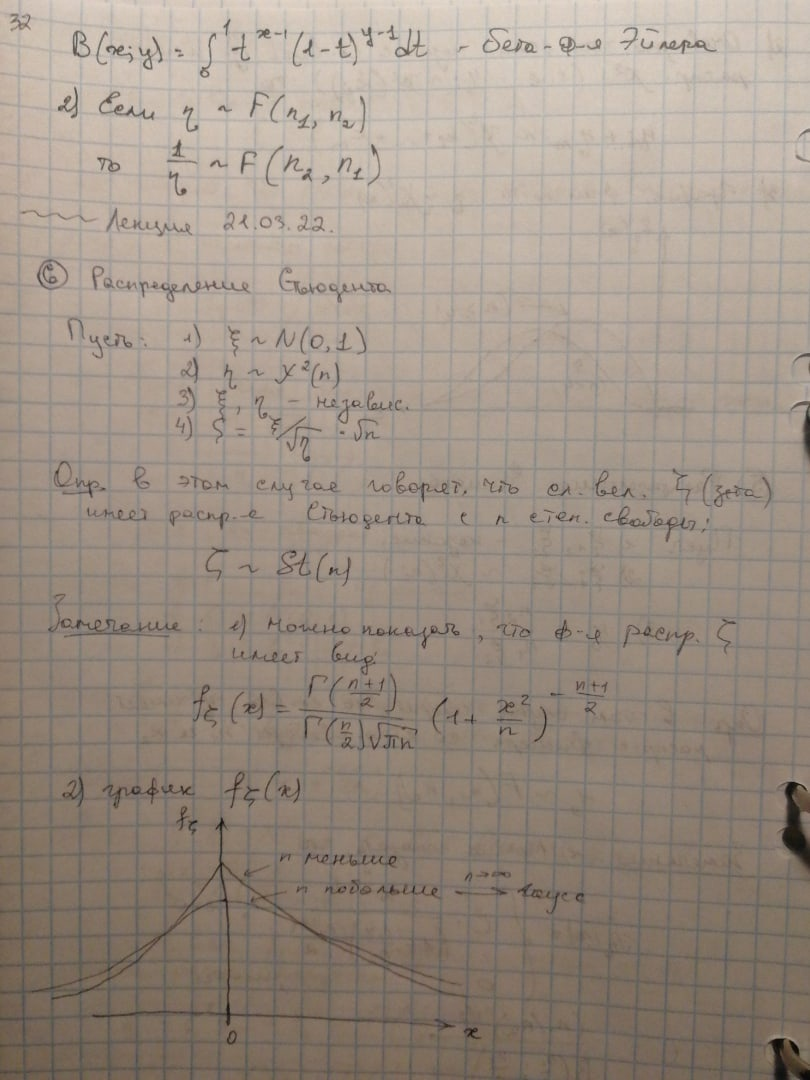
\includegraphics[scale=0.35]{1}}
	\caption{Схема работы суперблока}
\end{figure}


В данном примере мы рассмотрим раздел жёсткого диска (раздел вторичной памяти) с файловой системой ext2 (родная файлова система linux).

Блок - минимальная адресуемая единица физического носителя (вторичной памяти). В разных системах размер может отличаться. Каждый блок имеет уникальный адрес.

Любая файловая система предназначена для обеспечения долговременного хранения и доступа к файлам. Без доступа все это не нужно. Кроме того, что файловая система предназначена для хранения информации, однако в первую очередь она должна обеспечивать доступ к этой информации. Доступ - многоуровневый (вторичная память - внешнее устройства) на каком-то последнем этапе происходит обращение к устройству.

inode описывают физический файл, и они же так называемые дисковые inodeы содержат информацию об адресных блоках вторичной памяти, в которой находится файл, который описывается конкретным inodом.

Очевидно, что суперблок должен содержиться список inodов, но он должен содержать первый inode - inode корневого каталога.

Файловая система ext2 существует достаточное большое количество времени по причине того, что она хорошо написана. Данная система обеспечивает хранение и доступ к очень большим файлам. По аналогии с физическим адресным пространством оперативной памяти, если первые операционные системы требовали. чтобы процессу было выделено непрерываное адресное пространство, и это оказалось невозможным при быстром росте прикладного ПО. Такое требование в современных системах физически обеспечить невозможно. Не существует достаточно большого объекма физической памяти для обеспечения одновременной работы большого объема фзической памяти для обеспечения одновременной работы большого количества приложений с высокими требования к физической памяти, что характерно и для файлов. Размеры файлов также постоянно растут. Это было понято разработчиками Linux/Unix. Ими было предложено решение, когда файлу выделялось не непрерывное адресное пространство, а была обеспечена возможность выеления свободных участков адресного пространства. В результате было обеспечено хранение и доступ к файлам очень большого размера.

Практически все источники приводят эту информацию о файловой системе ext2 как наиболее яркий пример работы с файлами очень большого размера. 

Видно, что суперблок хранит информации о inodах, обеспечивая доступ к дисковому inodу, а дисковый inode хранит информацию об адресных блоках вторичной памяти, в которых располагается данные данного файла.

В этой файловой системы существует несколько типов адресации - прямая, косвенная, двойная косвенная и тройная косвенная.

Для адресов 12 блоов (0 - 11) используются для прямой адресации. Соответственно это непосредственно адрес информационного блока.

Следующие блоки содержат косвенные ссылки (indirect block). Этот блок содержит адреса инфомационных блоков.

struct super\_block\\
\{\\
	struct list\_head head s\_list;\\
	dev\_t s\_dev;\\
	unsigned long s\_blocksize;\\
	struct file\_system\_type *s\_type;\\
	unsigned long s\_flags;\\
	unsigned long s\_magik;\\
	struct dentry *s\_root;\\
	struct rw\_semaphore s\_unmount;\\
	...\\
	struct list\_head s\_mount;\\
	struct block\_device *s\_bdev;\\
	
	const struct dentry\_operations *s\_d\_op;\\
	...\\
	/* s\_node\_list\_lock protects s\_inode*/\\
	spin\_lock\_t s\_inode\_list\_lock;\\
	struct list\_head s\_inodes;\\
	...\\
	struct list\_head s\_inodes\_wb;\\
\};\\

Суперблоки объединены в спискок. В системе будет существовать столько суперблоков, сколько смонтировано файловых систем. При этом может быть смонтировано несколько файловых систем одного и того же типа, поэтому первое поле представляет из себя список.

Очевидно, что смотированая файловая система должна находиться на каком-то девайсе или на части ос, на части адресного пространство оперативной памяти или на внешнем устройства (это должен быть физический носитель) - второе поле.

Важное значение имеет размер блока (он является минимальной адресной единицей на вторичной памяти) - третье поле.

Тип файловой системы - важнейшее понятие в Linux, так как может поддерживать большое количество файловых систем. Структура file\_system\_type предназначена для регистрации типа конкретной файловой системы:\\
Есть флаги для работы с файловой системой\\
Есть магическое число для обеспечения надёжной работы\\
Указатель на root\\
Семафоры для чтения-записи\\

На суперблоке определён набор операций, которые с ним можно выполнять - struct super\_operations. В любой из перечисленных структур есть ссылка на операции, которые могут выполняться на этом суперблоке, фактически таблицу. Дентри являеся элементом пути к файлу. Каждый элемент пути имеет элемент inode и хранится на диске. Каждая структура содержит средства взаимоисключения. Список inodов должен защищаться, для этого используется спинлок.

Кроме этого есть список inodов. В этом списке находятся все inodы - дескрипторы физических файлов, созданных в конкретной файловой системе. 

s\_inodes\_wb - Write Back inodes, список грязных inodов. Грязным файлом называется изменённое значение.\\
struc super\_operations\\
\{\\
	struct inode *(*alloc\_inode)(struct super\_block *sb);\\
	void (*destroy\_inode)(struct inode *);\\
	void (*free\_inode)(struct inode *);\\
\};\\

Очевидно, что поскольку любая файловая система предназначена для хранения физических данных. Причём не просто данных, а поименованных. Мы видим, что это работа с inodом.